\documentclass[tikz, border=10pt]{standalone}
\usepackage{iftex}
\ifluatex
  \usepackage{fontspec}
  \usepackage{unicode-math}
  \setmainfont{Fira Sans}
  \setmonofont{Fira Mono}
  \setmathfont{Fira Math}
  % Fallback only for set-difference glyphs missing in Fira Math.
  \setmathfont{STIX Two Math}[range={"29F5,"2216}]
\else
  \usepackage[T1]{fontenc}
\fi

\usepackage{amsmath}
\usepackage{tikz}
\usetikzlibrary{arrows.meta}
\tikzset{every node/.style={font=\Large}}

% Theme toggle: set \darkbgfalse for light background preview.
\newif\ifdarkbg
\darkbgfalse
\ifdarkbg
  \colorlet{axiscol}{white}
  \colorlet{gridcol}{white!30!black}
  \colorlet{ticklabelcol}{white}
  \colorlet{funcol}{yellow!85!white}
\else
  \colorlet{axiscol}{black}
  \colorlet{gridcol}{black!25!white}
  \colorlet{ticklabelcol}{black}
  \colorlet{funcol}{blue!70!black}
\fi

% x: -3 to 1  (4 units)   xscale=1.3 → ~5.2 cm wide
% y: -8 to  8  (16 units)  yscale=0.55 → ~8.8 cm tall
% Elegant: f(-3) = (-2)^3 = -8  and  f(1) = 2^3 = 8
%          → the curve exits at the exact corners of the window.
\begin{document}
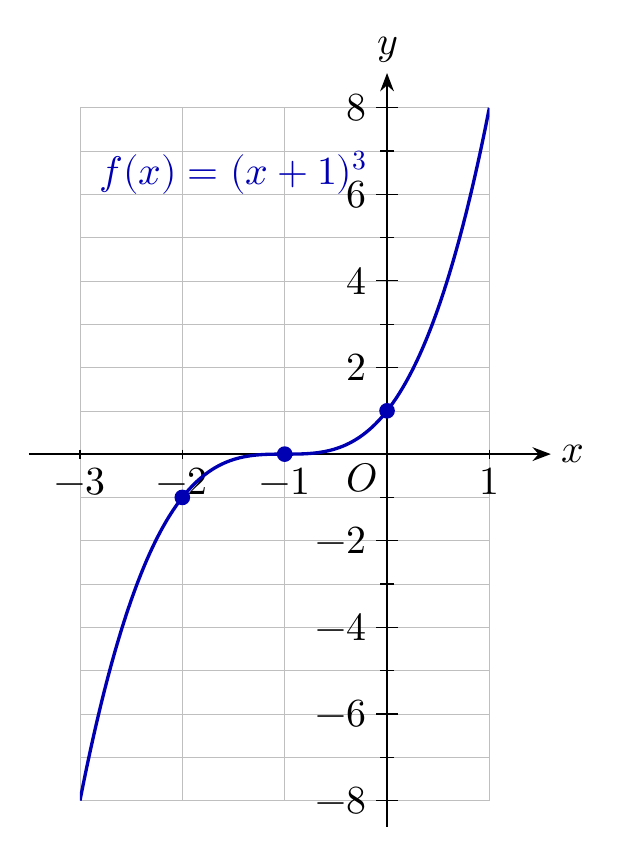
\begin{tikzpicture}[xscale=1.3, yscale=0.55, >=Stealth]

  % Cartesian grid.
  \draw[step=1, very thin, gridcol] (-3,-8) grid (1,8);

  % Axes.
  \draw[->, thick, axiscol] (-3.5,0) -- (1.6,0)
    node[right, text=axiscol] {$x$};
  \draw[->, thick, axiscol] (0,-8.6) -- (0,8.8)
    node[above, text=axiscol] {$y$};

  % Tick marks — x axis.
  \foreach \x in {-3,-2,-1,1} {
    \draw[axiscol] (\x, 3pt) -- (\x, -3pt)
      node[below, text=ticklabelcol] {$\x$};
  }

  % Tick marks — y axis (labelled every 2, minor every 1).
  \foreach \y in {-8,-6,-4,-2,2,4,6,8} {
    \draw[axiscol] (3pt,\y) -- (-3pt,\y)
      node[left, text=ticklabelcol] {$\y$};
  }
  \foreach \y in {-7,-5,-3,-1,1,3,5,7} {
    \draw[axiscol] (2pt,\y) -- (-2pt,\y);
  }

  % Origin label.
  \node[below left, text=axiscol] at (0,0) {$O$};

  % Function curve: f(x) = (x+1)^3, clipped to the plot window.
  \begin{scope}
    \clip (-3,-8) rectangle (1,8);
    \draw[domain=-3:1, smooth, very thick, funcol, samples=80]
      plot (\x, {(\x+1)^3});
  \end{scope}

  % Function label — upper-left, away from the curve.
  \node[right, text=funcol] at (-2.9,6.5) {$f(x)=(x+1)^3$};

  % Inflection point / root.
  \node[circle, fill=funcol, inner sep=2pt] at (-1,0) {};

  % y-intercept (0, 1).
  \node[circle, fill=funcol, inner sep=2pt] at (0,1) {};

  % Symmetric companion point (-2, -1).
  \node[circle, fill=funcol, inner sep=2pt] at (-2,-1) {};

\end{tikzpicture}
\end{document}
